\subsection{Edge processing}

\subsubsection{Problem definition}

The depth image has a smaller resolution than the RGB image. There is no direct correspondence between a pixel in the RGB image and its corresponding depth. This correspondence is handled by the SDK provided by Microsoft. Therefore, the associated depth of the RGB pixel could be wrong. This is probably one of the reasons of the noise in the edges. Some of the resulting 3D points can represent the background. Having some background points in the middle of the face is disturbing and has to be handled. To handle in part this problem, some image processing techniques are applied to the depth image of both cameras independently.

% \begin{figure}[H]
% \centering
%   \begin{subfigure}[b]{0.35 \textwidth}
%     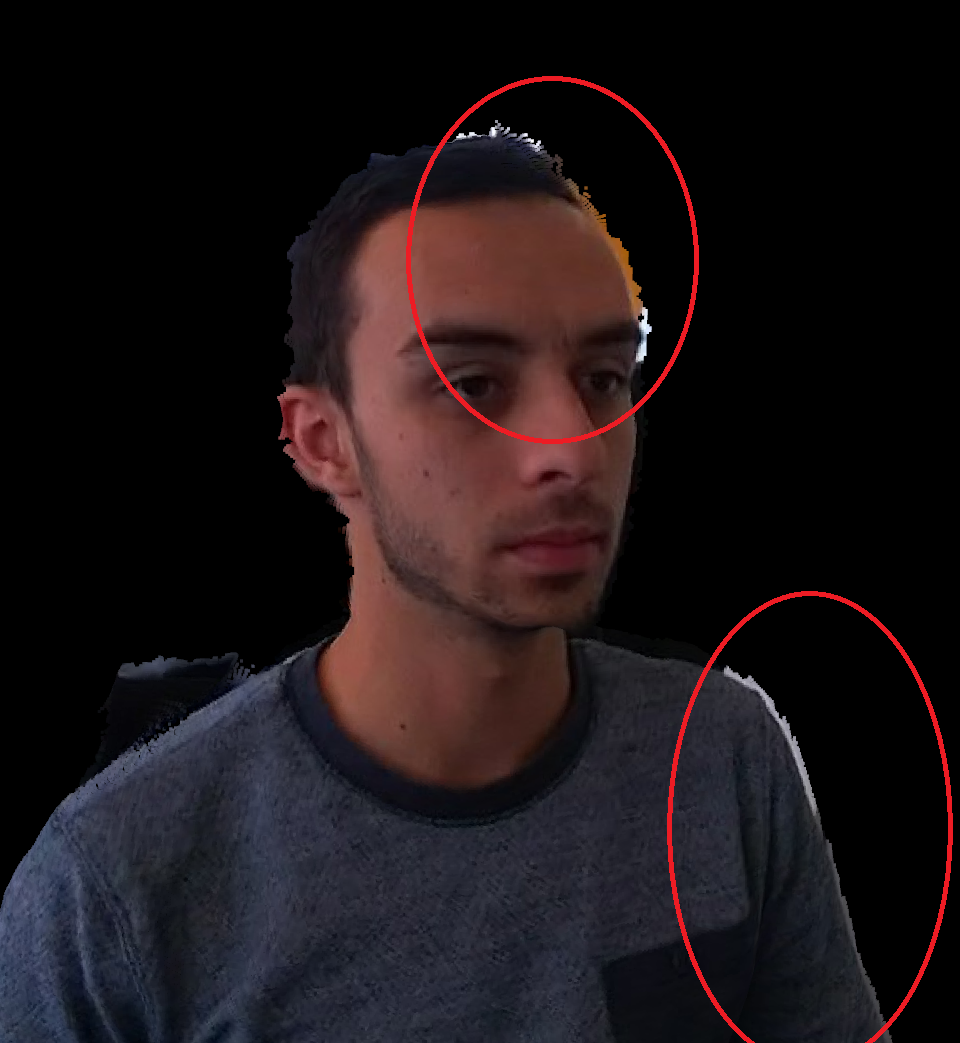
\includegraphics[width=\textwidth]{images/visual_enhancement/edge/face_white_noise_red.png}
%     \caption{Edge artefacts in point cloud}
%     \label{figure:face_white_noise_red}
%   \end{subfigure}
%   \hfill
%   \begin{subfigure}[b]{0.35 \textwidth}
%     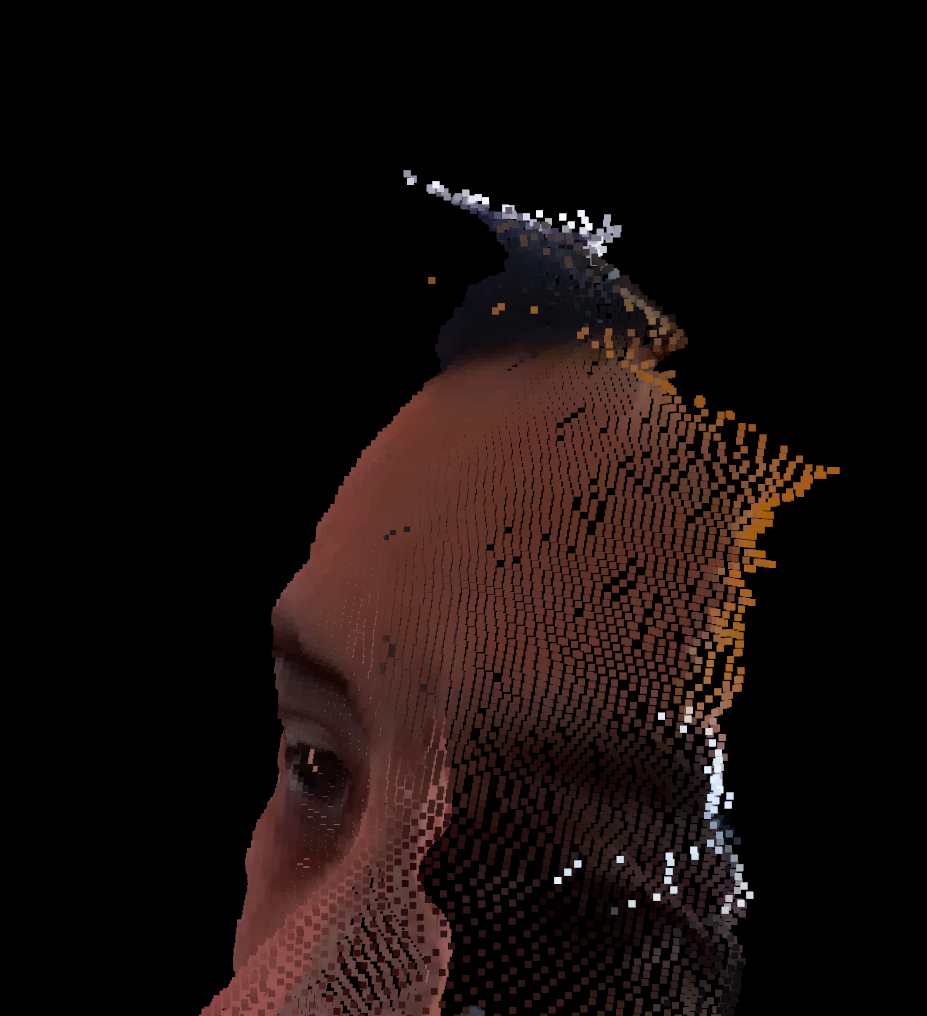
\includegraphics[width=\textwidth]{images/visual_enhancement/edge/white_noise.png}
%     \caption{Zoom on edge artefacts}
%     \label{figure:white_noise}
%   \end{subfigure}
%   \caption{Edge artefacts are visible in the point clouds. These white and yellow points come from the background.}
%   \label{figure:edge_artefact}
% \end{figure}


% \begin{figure}[!ht]
% \begin{multicols}{2}
%         \begin{subfigure}{\linewidth}
%               \centering
%                 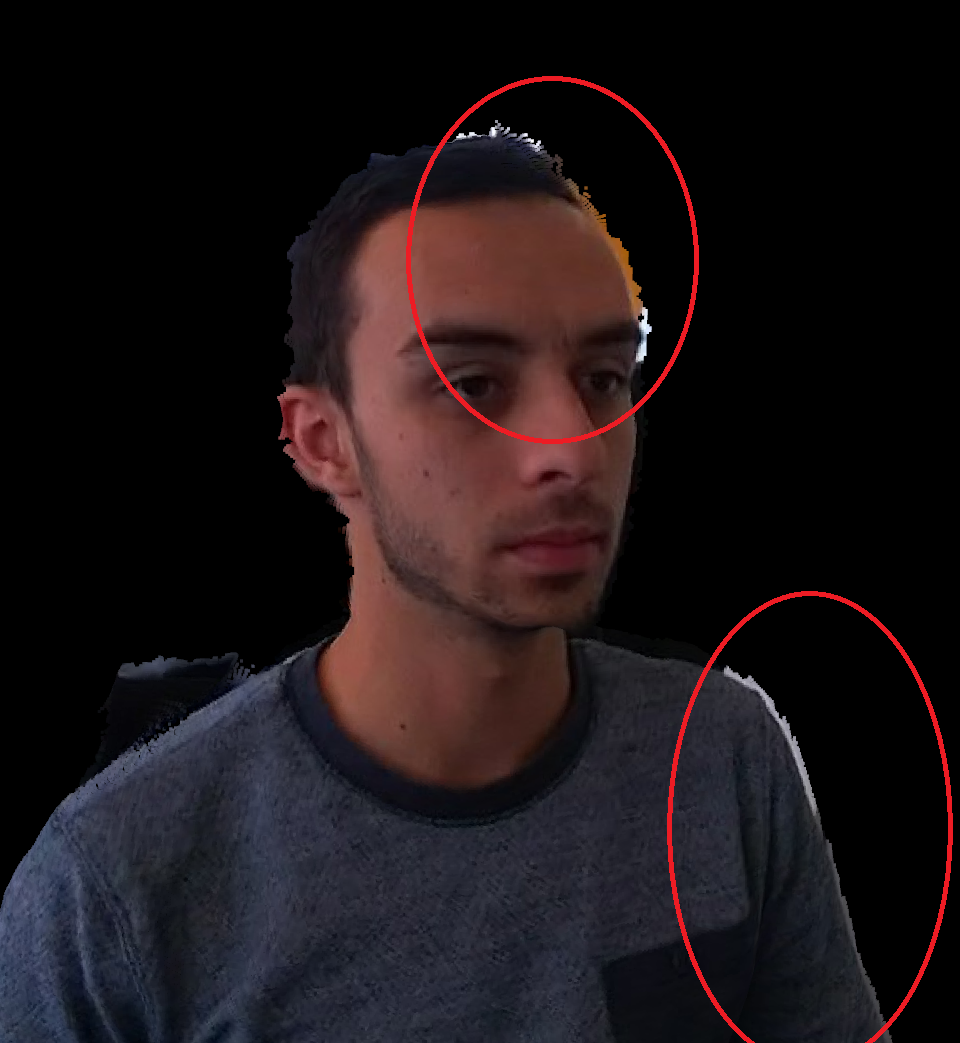
\includegraphics[width=.8\linewidth]{images/visual_enhancement/edge/face_white_noise_red.png}
%               \caption{Edge artefacts in point cloud}
%               \label{figure:face_white_noise_red}
%         \end{subfigure}
%         \begin{subfigure}{\linewidth}
%               \centering
%              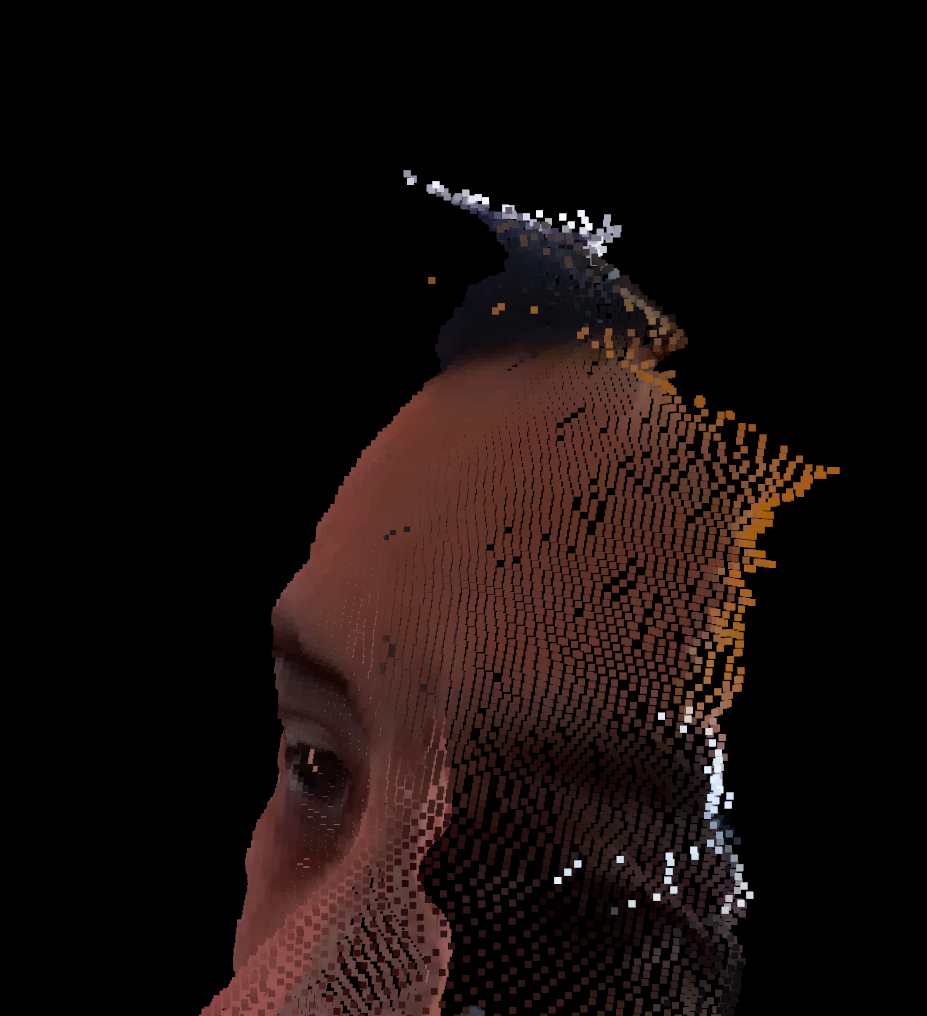
\includegraphics[width=.8\linewidth]{images/visual_enhancement/edge/white_noise.png}
%               \caption{Zoom on edge artefacts}
%               \label{figure:white_noise}
%         \end{subfigure}
% \end{multicols}\vspace{-10pt}
% \caption{Edge artefacts are visible in the point clouds. These white and yellow points come from the background.}
% \label{figure:edge_artefact}
% \end{figure}

\begin{figure}[!ht]

\begin{multicols}{2}
        \begin{subfigure}{\linewidth}
               \centering
                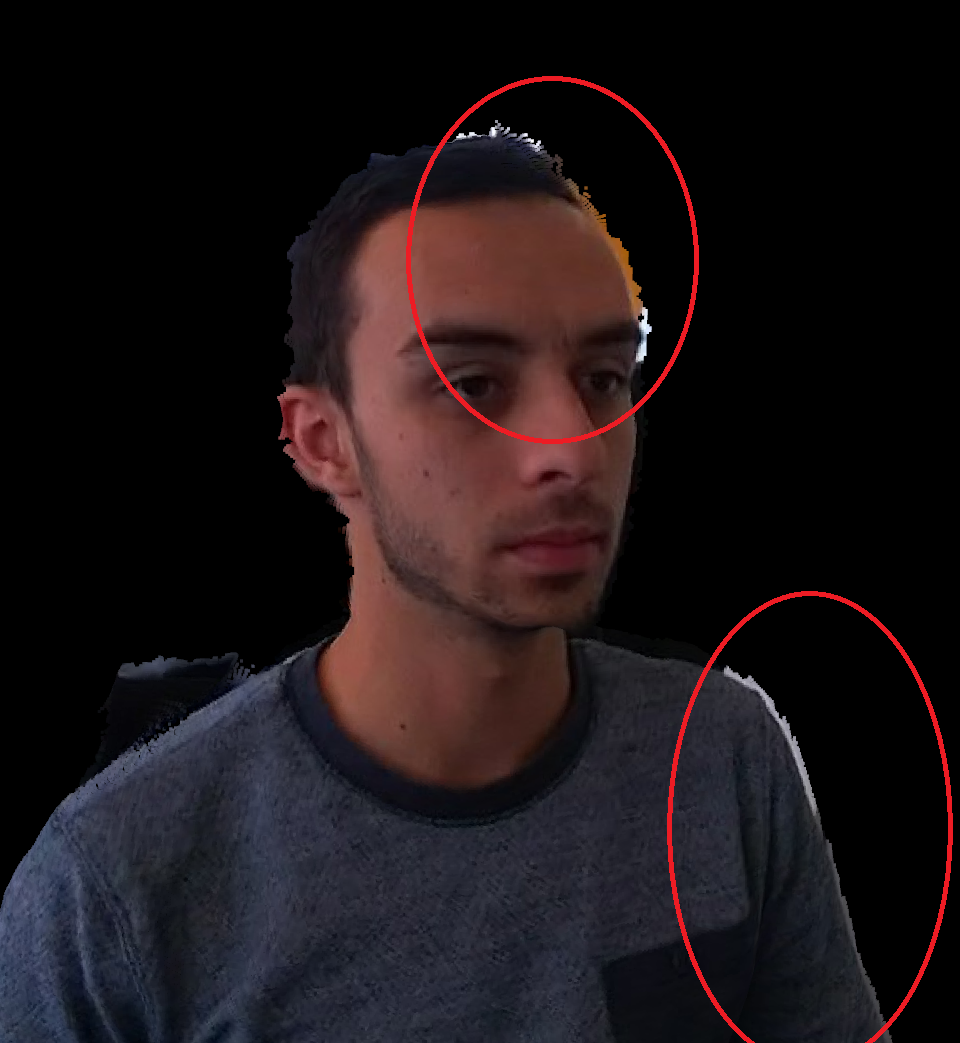
\includegraphics[width=.8\linewidth]{images/visual_enhancement/edge/face_white_noise_red.png}
               \caption{Edge artefacts in point cloud}\label{figure:face_white_noise_red}
        \end{subfigure}
        
        
        \begin{subfigure}{\linewidth}
               \centering
             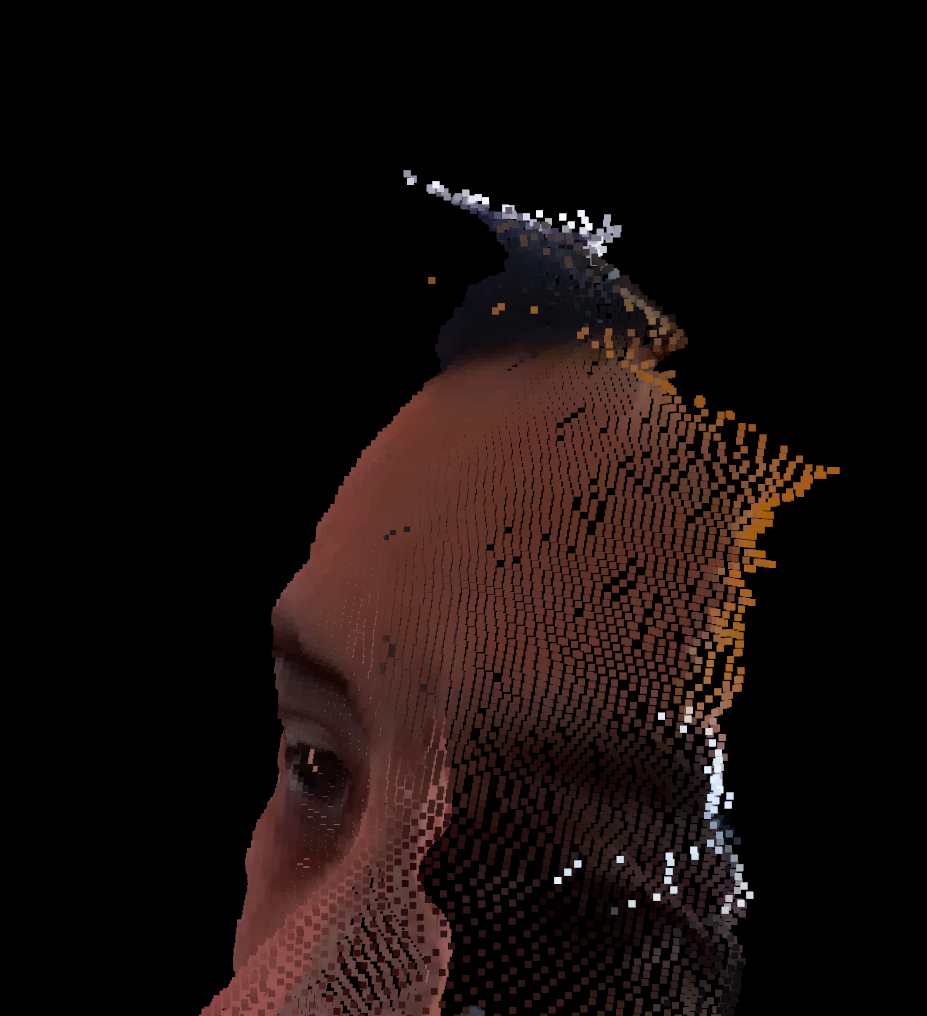
\includegraphics[width=.8\linewidth]{images/visual_enhancement/edge/white_noise.png}
               \caption{Zoom on edge artefacts}\label{figure:white_noise}
        \end{subfigure}
\end{multicols}\vspace{-10pt}
\caption{Edge artefacts are visible in the point clouds. These white and yellow points come from the background.}
\label{figure:edge_artefact}

\end{figure}


\subsubsection{Proposed method}

To correct some of the undesirable effects that appear on the edges, the depth image is modified for each frame. First, a mask of the foreground scene is created based on the distance information available in the depth image. Then, an erode morphological operation with a square kernel is applied on the mask to erode its borders. The resulting positive region of the mask is then smaller than the original one. This 'eroded' mask is then multiplied to the original corresponding depth image. It results in a depth image of the foreground scene with eroded edges. This depth image is then used to create the point cloud of the foreground scene. The pseudocode of the edge erosion process is detailed in algorithm \ref{algo:erosion}. Figure \ref{figure:edge_pipeline} shows the pipeline of the whole procedure.

\begin{algorithm}
    \caption{Edge erosion algorithm}
    \label{algo:erosion}
    \begin{algorithmic}[1] % The number tells where the line numbering should start
        \Procedure{Edge-Erosion}{$capturedDepthFrame, distMin, distMax$}
            \State $depthImage\gets capturedDepthFrame$
            \State  $depthImageInRange \gets$ selectRange($depthImage, distMin, distMax$) \Comment{Foreground}
            \State $mask\gets$ Transform $depthImageInRange$ in a binary mask of the foreground
            \State $erodedMask\gets$ ErosionMorphological($mask$) \Comment{Erosion of the foreground mask}
            \State $depthProcessed\gets$ $capturedDepthFrame$ * $erodedMask$
            \newline
            \State \textbf{return} $depthProcessed$ \Comment{Eroded depth image of the foreground}
        \EndProcedure
    \end{algorithmic}
\end{algorithm}


\begin{figure}[H]
    \centering
    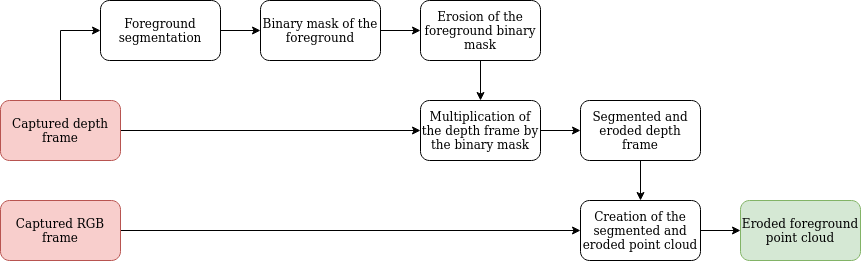
\includegraphics[width=0.95\textwidth]{images/visual_enhancement/edge/edge_pipeline.png}
    \caption{Pipeline of the edge processing procedure. Input: Captured depth frame \& Captured RGB frame. Output: Eroded foreground point cloud.}
    \label{figure:edge_pipeline}
\end{figure}




\subsubsection{Results}

This edge erosion algorithm is tested on a selected frame where the artefacts are visible, see figure \ref{figure:edge_artefact}. This evaluation is subjective.

\begin{figure}[H]
\centering
  \begin{subfigure}[b]{0.48 \textwidth}
    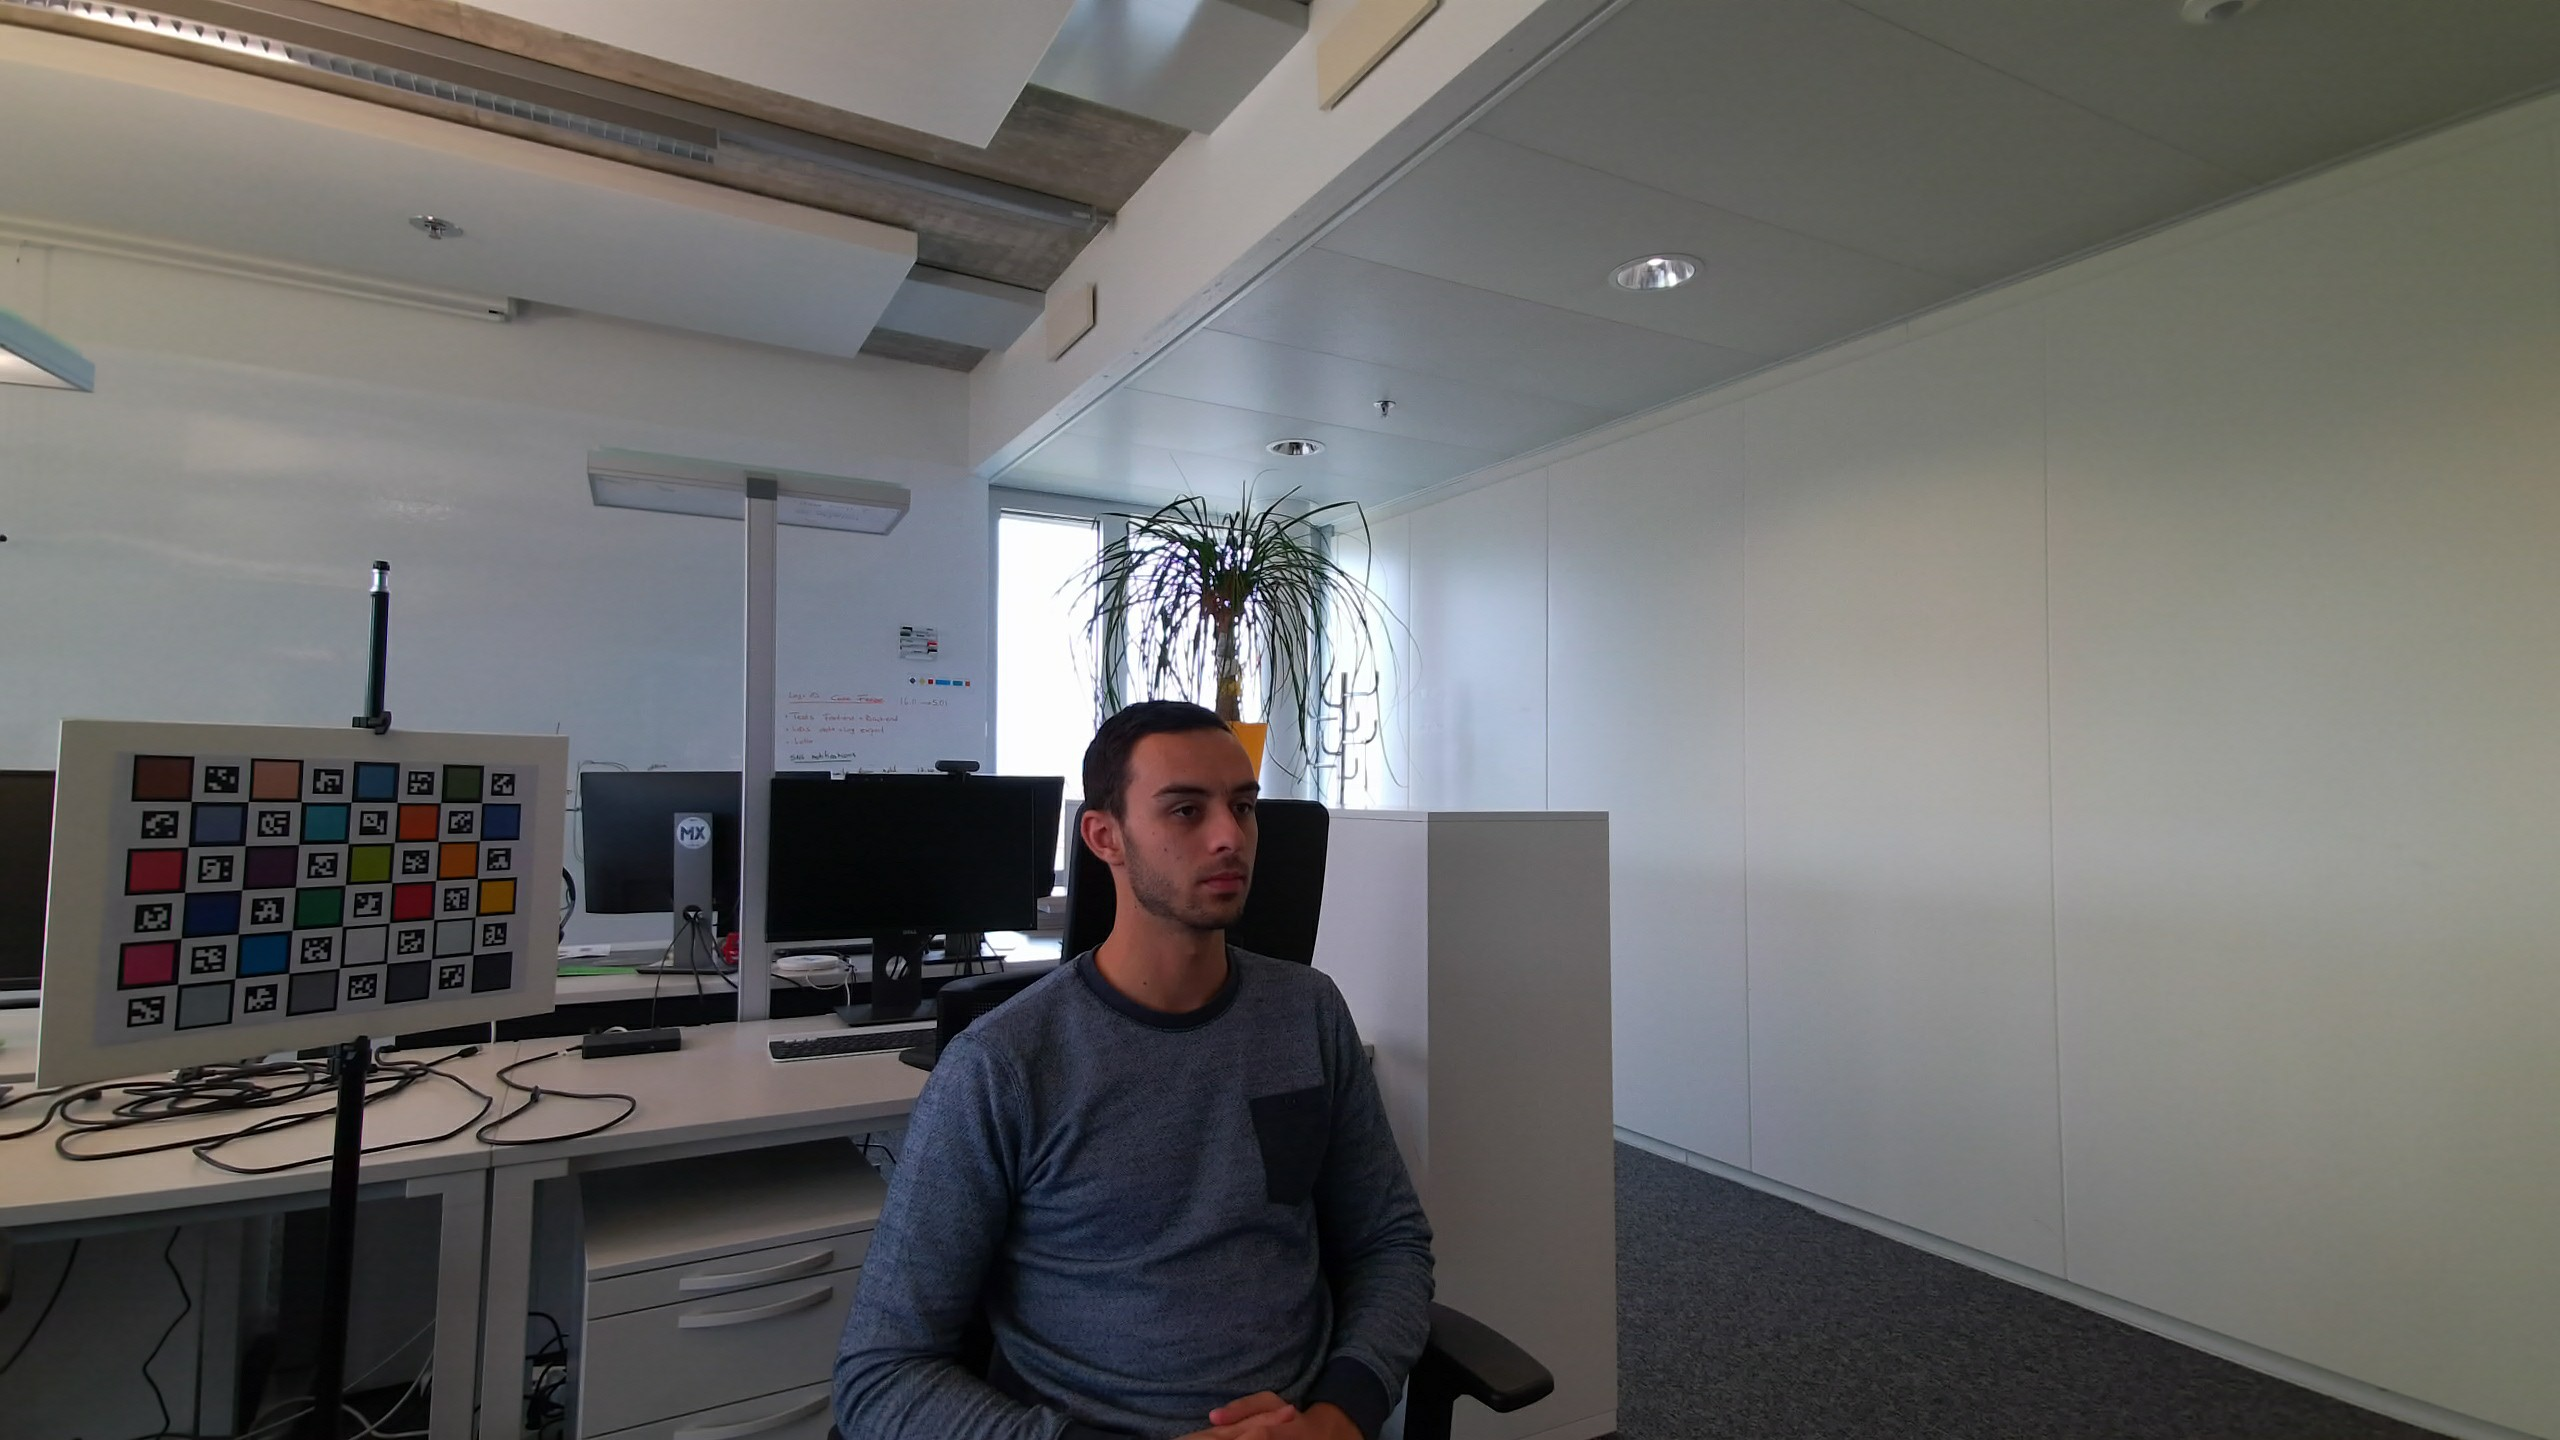
\includegraphics[width=\textwidth]{images/visual_enhancement/edge/sub_00150.jpg}
    \caption{Original RGB image}
    \label{figure:sub_00150_edge}
  \end{subfigure}
  \hfill
  \begin{subfigure}[b]{0.48 \textwidth}
    
\includegraphics[width=\textwidth]{images/visual_enhancement/edge/mask_2.png}
    \caption{Binary mask of the foreground scene}
    \label{figure:mask_2}
  \end{subfigure}
  \caption{RGB frame and its corresponding binary mask}
  \label{figure:Chessboard_detection}
\end{figure}

For this experiment, the selected depth range was set from 1000 mm to 1400 mm. Figure \ref{figure:mask_2} shows the resulting binary mask of the foreground created thanks to the original depth image, see figure \ref{figure:depth_colour}. Then an erosion morphological operator is applied on the binary mask. The original depth image is multiplied by the resulting 'eroded' mask. It results in a depth image of the foreground with eroded edges, see figure \ref{figure:depth_colour_processed}.

\begin{figure}[H]
\centering
  \begin{subfigure}[b]{0.48 \textwidth}
    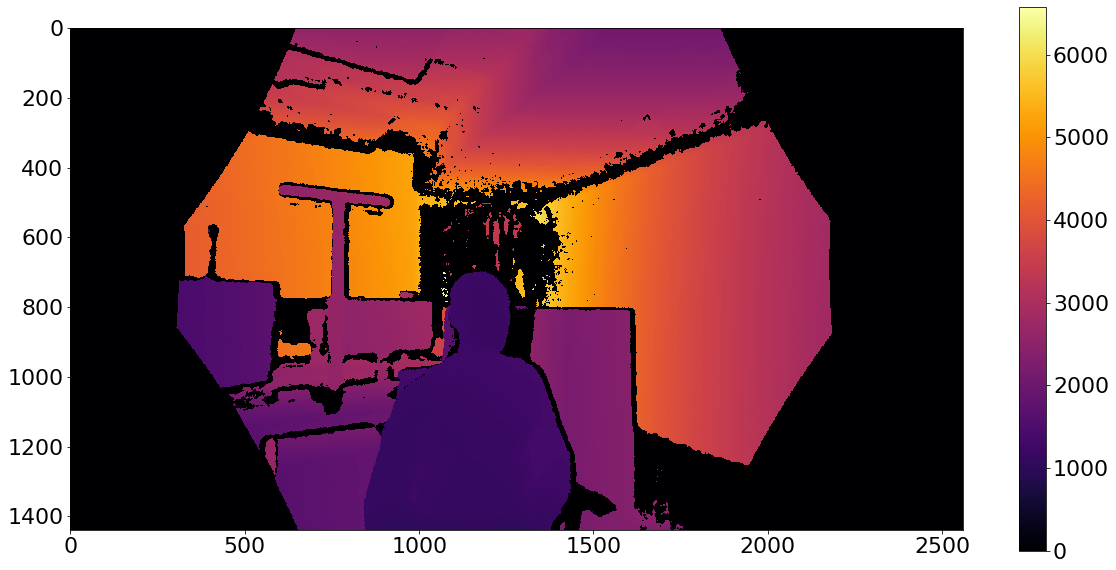
\includegraphics[width=\textwidth]{images/visual_enhancement/edge/depth_colour.png}
    \caption{Original depth image}
    \label{figure:depth_colour}
  \end{subfigure}
  \hfill
  \begin{subfigure}[b]{0.48 \textwidth}
    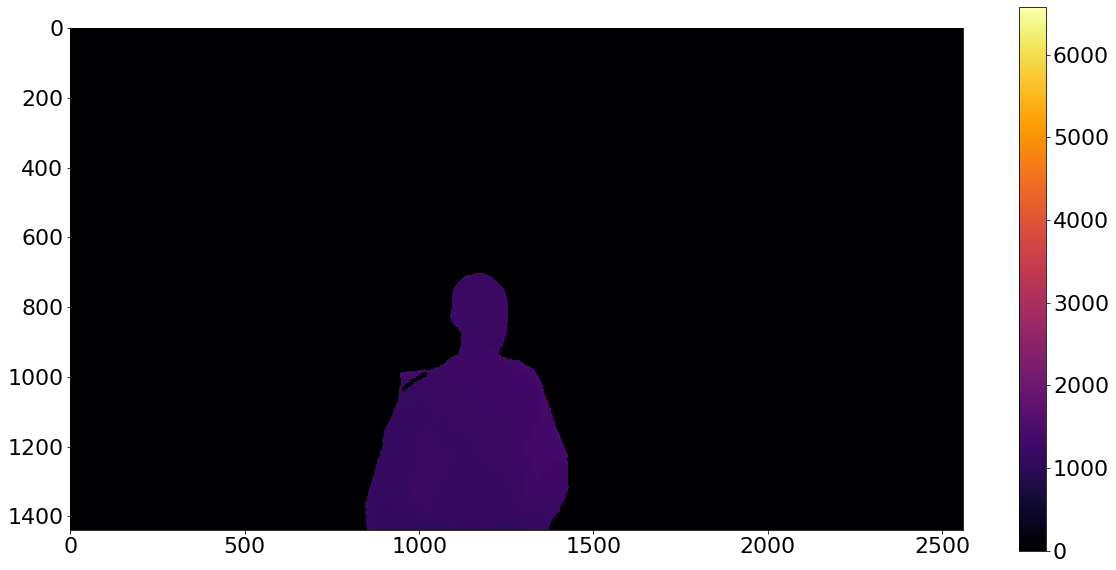
\includegraphics[width=\textwidth]{images/visual_enhancement/edge/dept_colour_processed.png}
    \caption{Depth image after multiplication by the eroded mask}
    \label{figure:depth_colour_processed}
  \end{subfigure}
  \caption{Depth image of the scene. The scale is in mm. Black parts represent the absence of depth information}
  \label{figure:dept_colour}
\end{figure}

The transformed depth image and the original RGB image are used to create the corresponding point cloud. It results in a point cloud with eroded edges. The points of the background are no more visible in the face, see figure \ref{figure:edge_result}. The non-desired artefacts have disappeared. 

% \begin{figure}[H]
% \centering
%   \begin{subfigure}[b]{0.35 \textwidth}
%     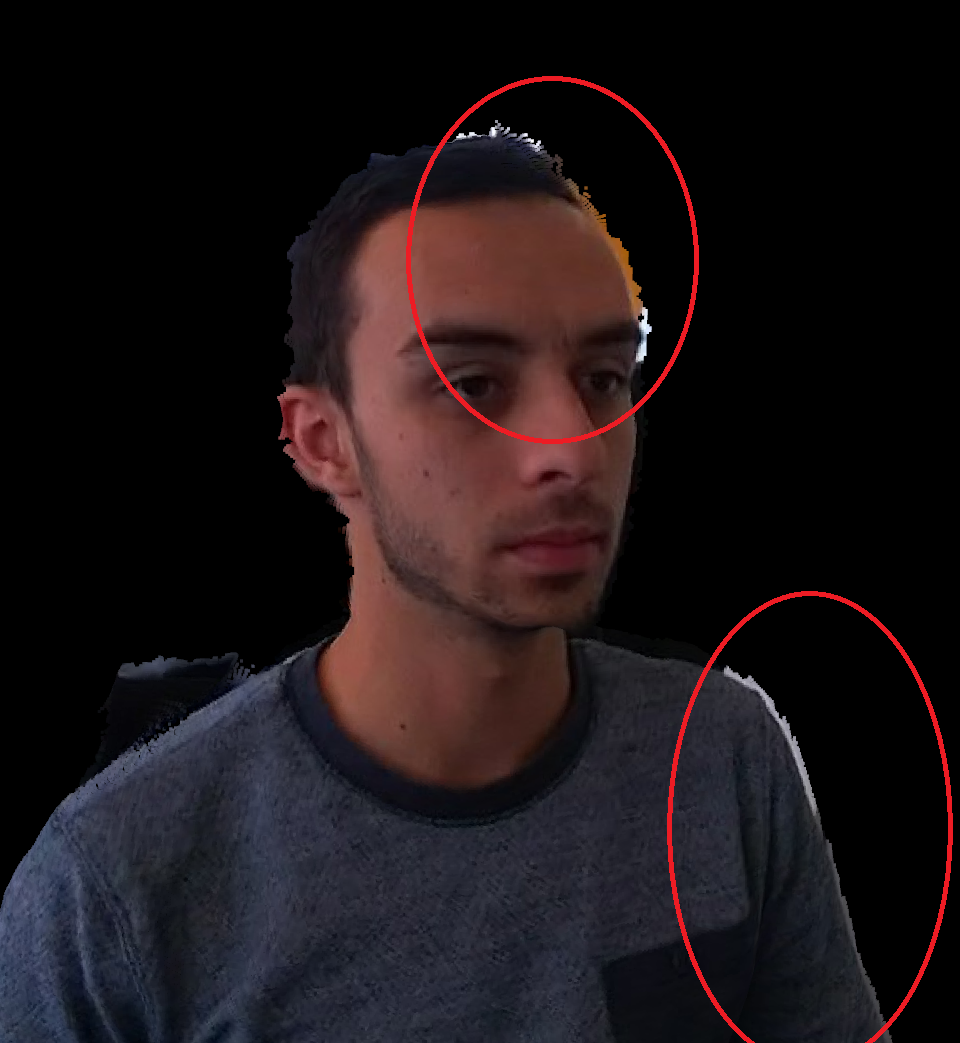
\includegraphics[width=\textwidth]{images/visual_enhancement/edge/face_white_noise_red.png}
%     \caption{Original foreground point cloud}
%     \label{figure:face_white_noise_red_2}
%   \end{subfigure}
%   \hfill
%   \begin{subfigure}[b]{0.35 \textwidth}
%     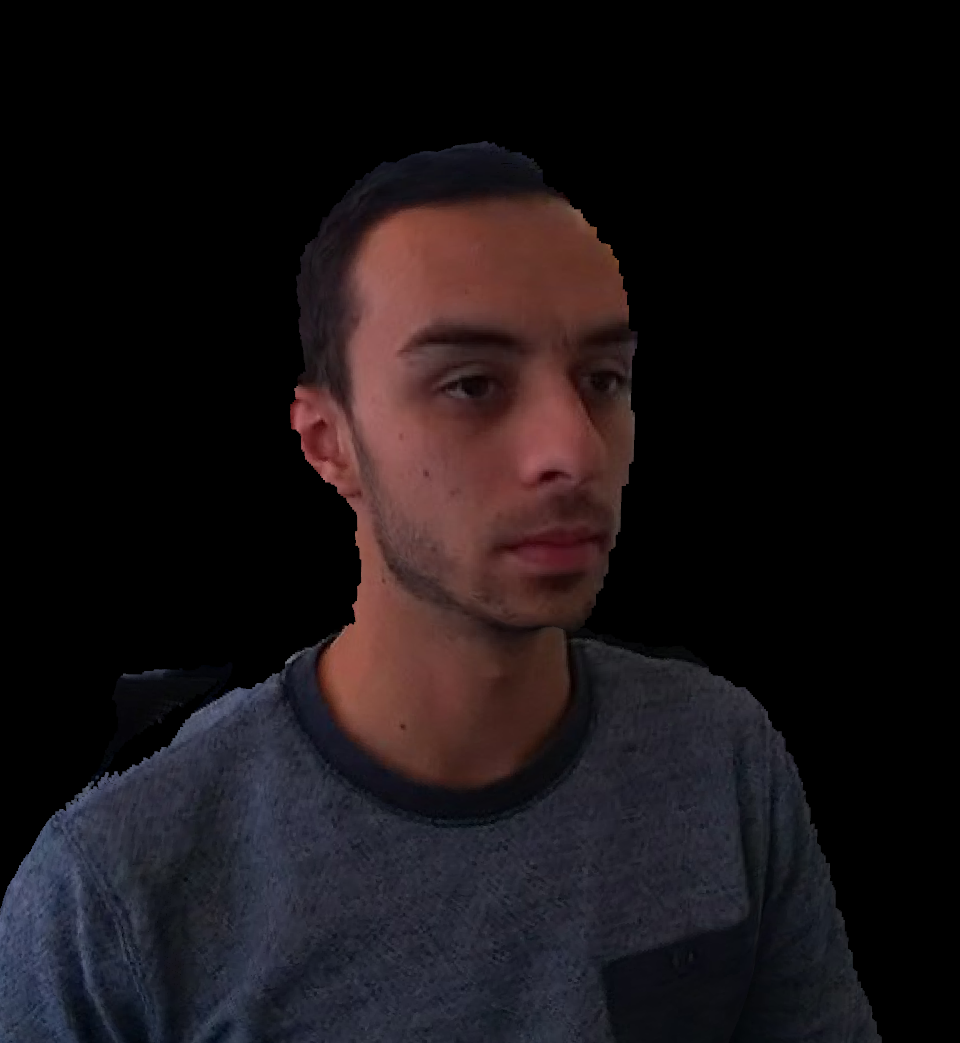
\includegraphics[width=\textwidth]{images/visual_enhancement/edge/eroded_face.png}
%     \caption{Eroded foreground point cloud}
%     \label{figure:eroded_face}
%   \end{subfigure}
%   \hfill
%   \begin{subfigure}[b]{0.35 \textwidth}
%     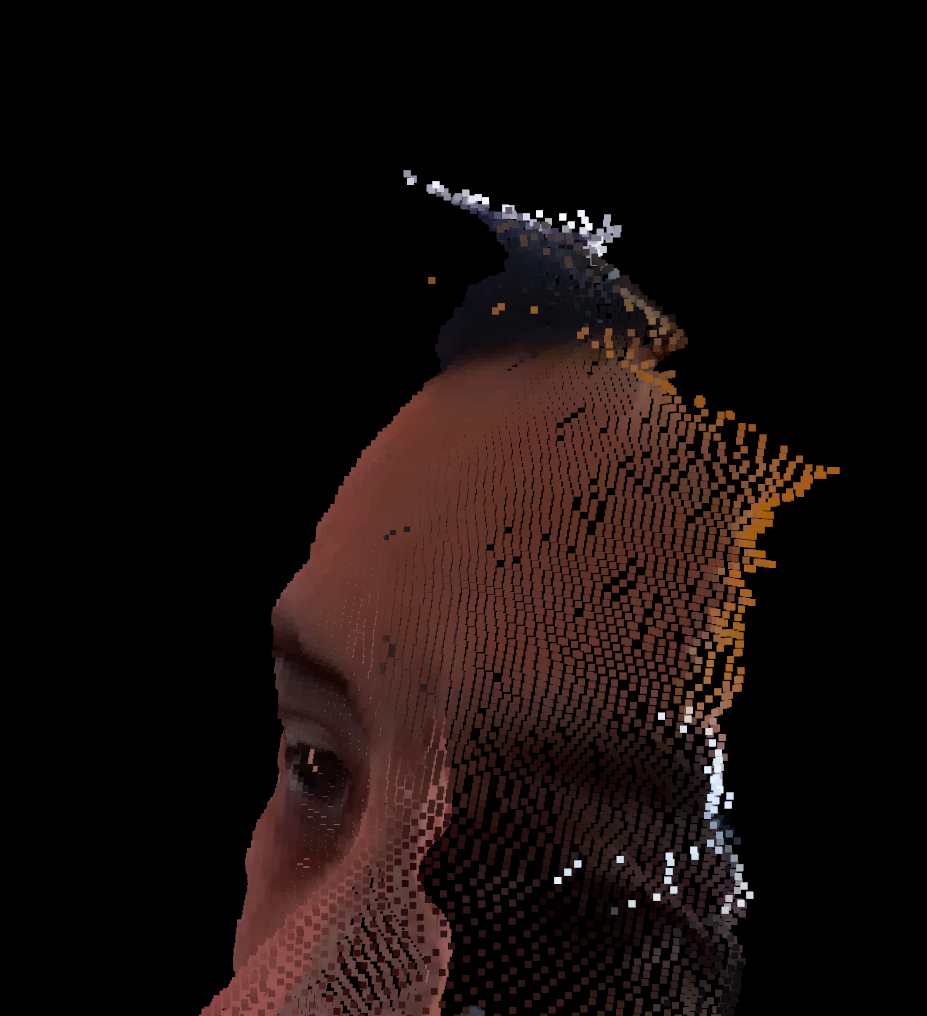
\includegraphics[width=\textwidth]{images/visual_enhancement/edge/white_noise.png}
%     \caption{Zoom on the original foreground}
%     \label{figure:white_noise_2}
%   \end{subfigure}
%   \hfill
%   \begin{subfigure}[b]{0.35 \textwidth}
%     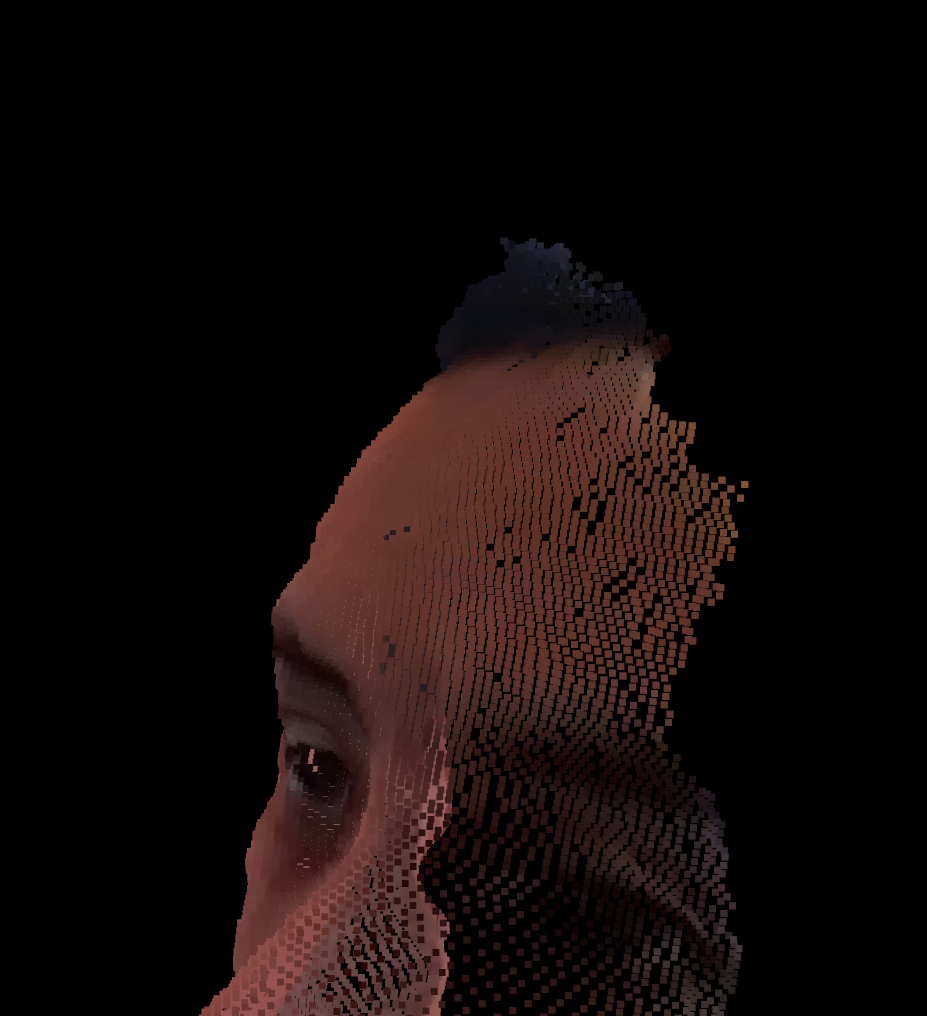
\includegraphics[width=\textwidth]{images/visual_enhancement/edge/eroded_noise_face.png}
%     \caption{Zoom on the eroded foreground}
%     \label{figure:eroded_noise_face}
%   \end{subfigure}
%   \caption{Selected point cloud before and after the application of the edge erosion algorithm}
%   \label{figure:edge_result}
% \end{figure}


\begin{figure}[!ht]

\begin{multicols}{2}
        \begin{subfigure}{\linewidth}
               \centering
                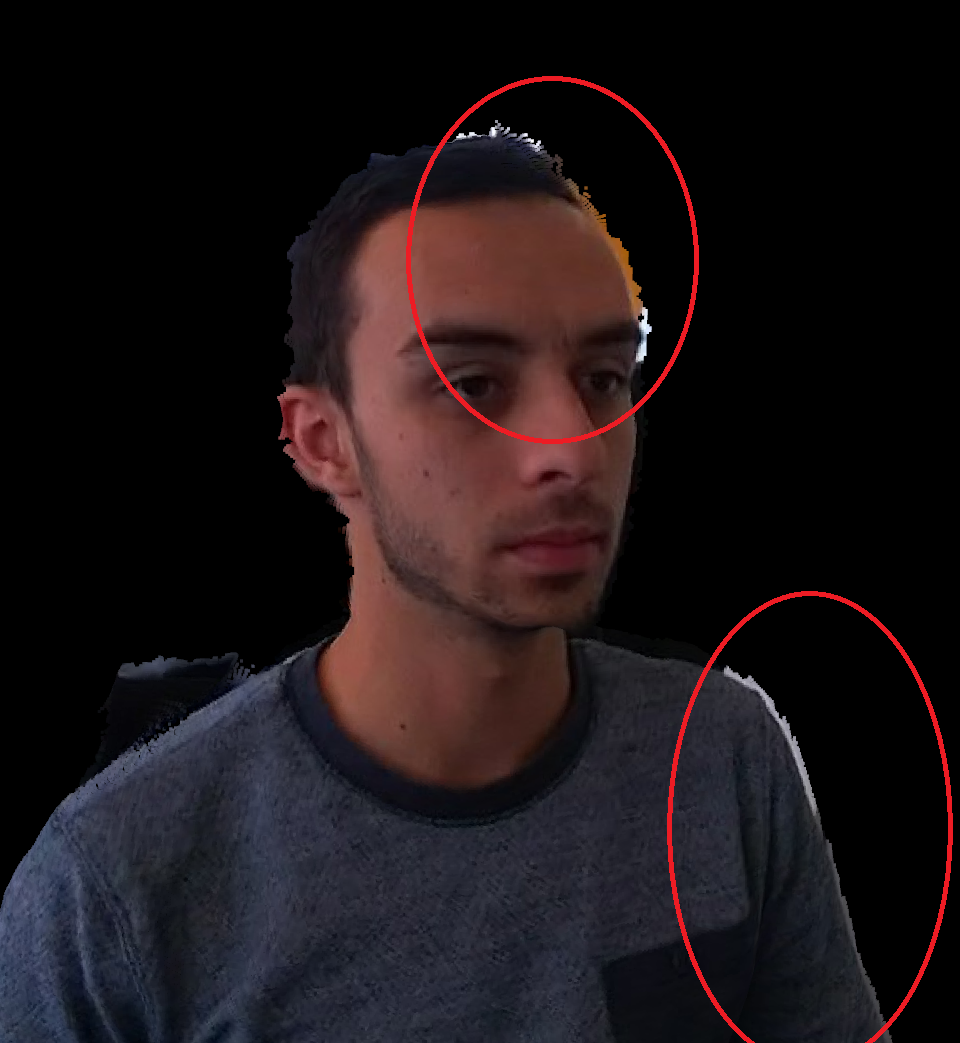
\includegraphics[width=.8\linewidth]{images/visual_enhancement/edge/face_white_noise_red.png}
               \caption{Original foreground point cloud}\label{figure:face_white_noise_red_2}
        \end{subfigure}
        
        
        \begin{subfigure}{\linewidth}
               \centering
             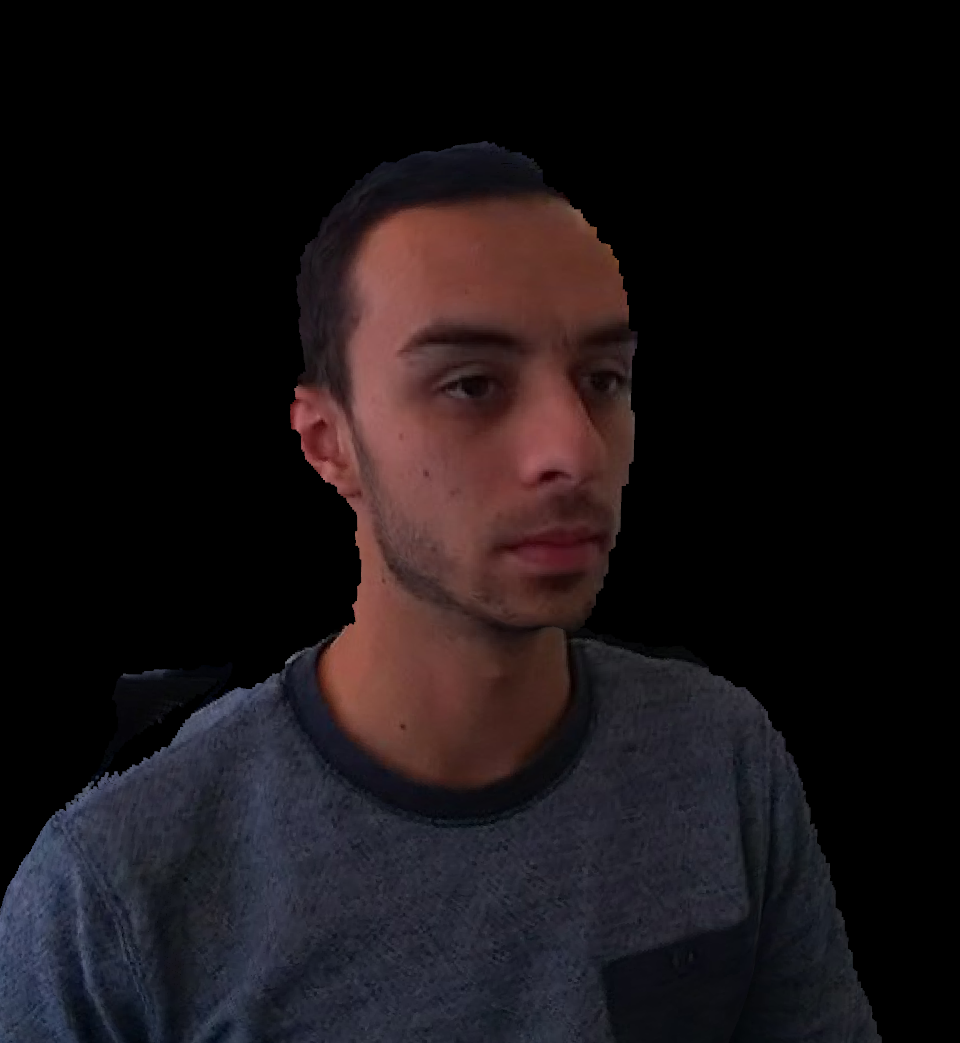
\includegraphics[width=.8\linewidth]{images/visual_enhancement/edge/eroded_face.png}
               \caption{Eroded foreground point cloud}\label{figure:eroded_face}
        \end{subfigure}
        
        
        \begin{subfigure}{\linewidth}
               \centering
             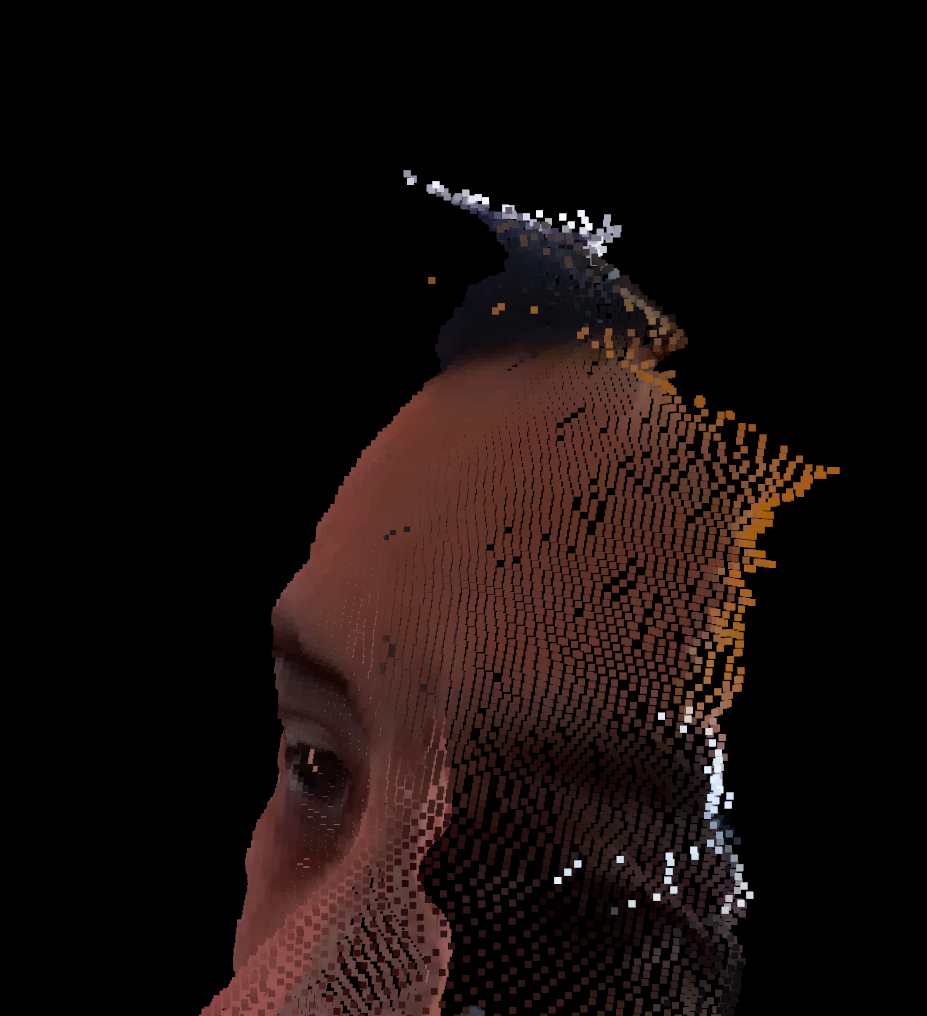
\includegraphics[width=.8\linewidth]{images/visual_enhancement/edge/white_noise.png}
               \caption{Zoom on the original foreground}\label{figure:white_noise_2}
        \end{subfigure}
        
        
        \begin{subfigure}{\linewidth}
               \centering
             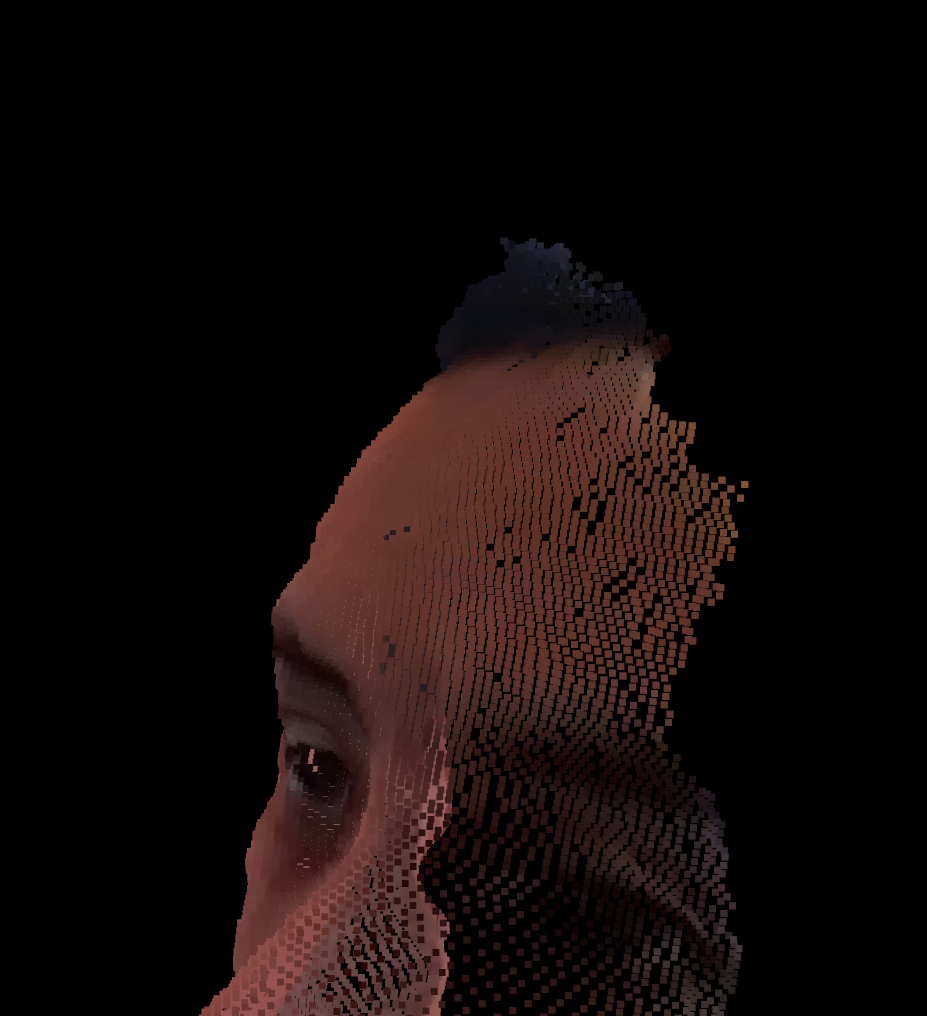
\includegraphics[width=.8\linewidth]{images/visual_enhancement/edge/eroded_noise_face.png}
               \caption{Zoom on the eroded foreground}\label{figure:eroded_noise_face}
        \end{subfigure}
\end{multicols}\vspace{-10pt}
\caption{Selected point cloud before and after the application of the edge erosion algorithm}
\label{figure:edge_result}

\end{figure}








\subsubsection{Discussion}

This edge erosion algorithm gives good results in a video point cloud stream. It improves the rendering of the scene. However, it has some limitations.  Because of the segmentation based on the depth distance, if an object is placed in front of the person, it will be merged in the binary mask and therefore its edges won't be eroded. A segmentation process based on object detection could be used instead to process the edges of each object/human independently. Another limitation is the fact that this process erodes also some parts that are not noise, it doesn't distinguish noise points from 'good' points.